\vspace{-0.06in}
\section{Related Work}
\subsection{Time Series Forecasting}
Time series forecasting has evolved from classical models like ARIMA, effective under ideal conditions \citep{box1968some,zhang2003time}, to modern deep learning approaches. 
% While ARIMA offers theoretical guarantees, it struggles with real-world data complexities. 
Machine learning methods \citep{chen2016xgboost,ke2017lightgbm} remain highly robust due to their interpretability and ability to model nonlinear relationships.  The advent of deep learning introduced sequence-to-sequence models such as Recurrent Neural Networks, which initially captured temporal dynamics well \citep{hewamalage2021recurrent,salinas2020deepar}. However, RNNs face limitations like restricted receptive fields and error accumulation \citep{salinas2020deepar}. Advanced architectures incorporating self-attention and convolutional networks have since been developed to capture long-range dependencies \citep{lai2018modeling,li2019enhancing}. Concurrently, integrating traditional techniques like trend-seasonal decomposition into neural networks has improved performance \citep{wen2020fast}. Notably, even simple linear networks enhanced with decomposition strategies can achieve competitive results \citep{zeng2023transformers}. Additionally, slice-based methods have shown promise in long-term forecasting by segmenting time series for better accuracy \citep{nie2022time,zhang2023crossformer}. These advancements blend classical principles with deep learning to tackle the challenges of TSF.

\vspace{-0.06in}

\subsection{LLM-based Time Series Forecasting}
In recent years, large language models (LLMs) have attracted attention for their ability to understand and generate human-like text, now extending into time series analysis \citep{zhang2024large,jiang2024empowering,jin2024position}. The application of LLMs in this field primarily follows two approaches: fine-tuning and prompt-based zero-shot learning. Fine-tuning involves further training pre-trained LLMs on specific time series data to improve performance \citep{chang2023llm4ts,chang2024align,liu2025calf,jin2023time}, though it requires significant labeled data. Conversely, prompt-based zero-shot methods utilize the model's existing knowledge through carefully designed prompts, avoiding task-specific training \citep{gruver2023large,liu2024lstprompt}.
% While more flexible and resource-efficient, these methods may not match the performance of fine-tuned models, especially in specialized tasks \citep{tang2025time,wang2024tabletime}.
More recently, LLM-based time series studies have moved beyond direct forecasting toward reasoning-oriented temporal understanding, exploring context-aware forecasting, time-series question answering, anomaly interpretation, and slow-thinking forecasting \citep{wang2025itformer,kong2025time, ni2026streasoner}. Along this direction, more complex frameworks further organize temporal reasoning around perception, extrapolation, decision-making, and pattern-aware question answering \citep{guan2025timeomni,lu2026patra, tao2026cast}.
These advances suggest that effective LLM-based time series modeling requires explicit alignment with temporal patterns and reasoning processes, motivating us to train LLMs with slow-thinking forecasting ability rather than relying solely on prompting or generic adaptation.

% Both paradigms illustrate the growing interest in using LLMs for time series, despite challenges in optimizing their inherent effectiveness and predictive accuracy for such tasks.
\begin{figure*}[t] 
    \centering
    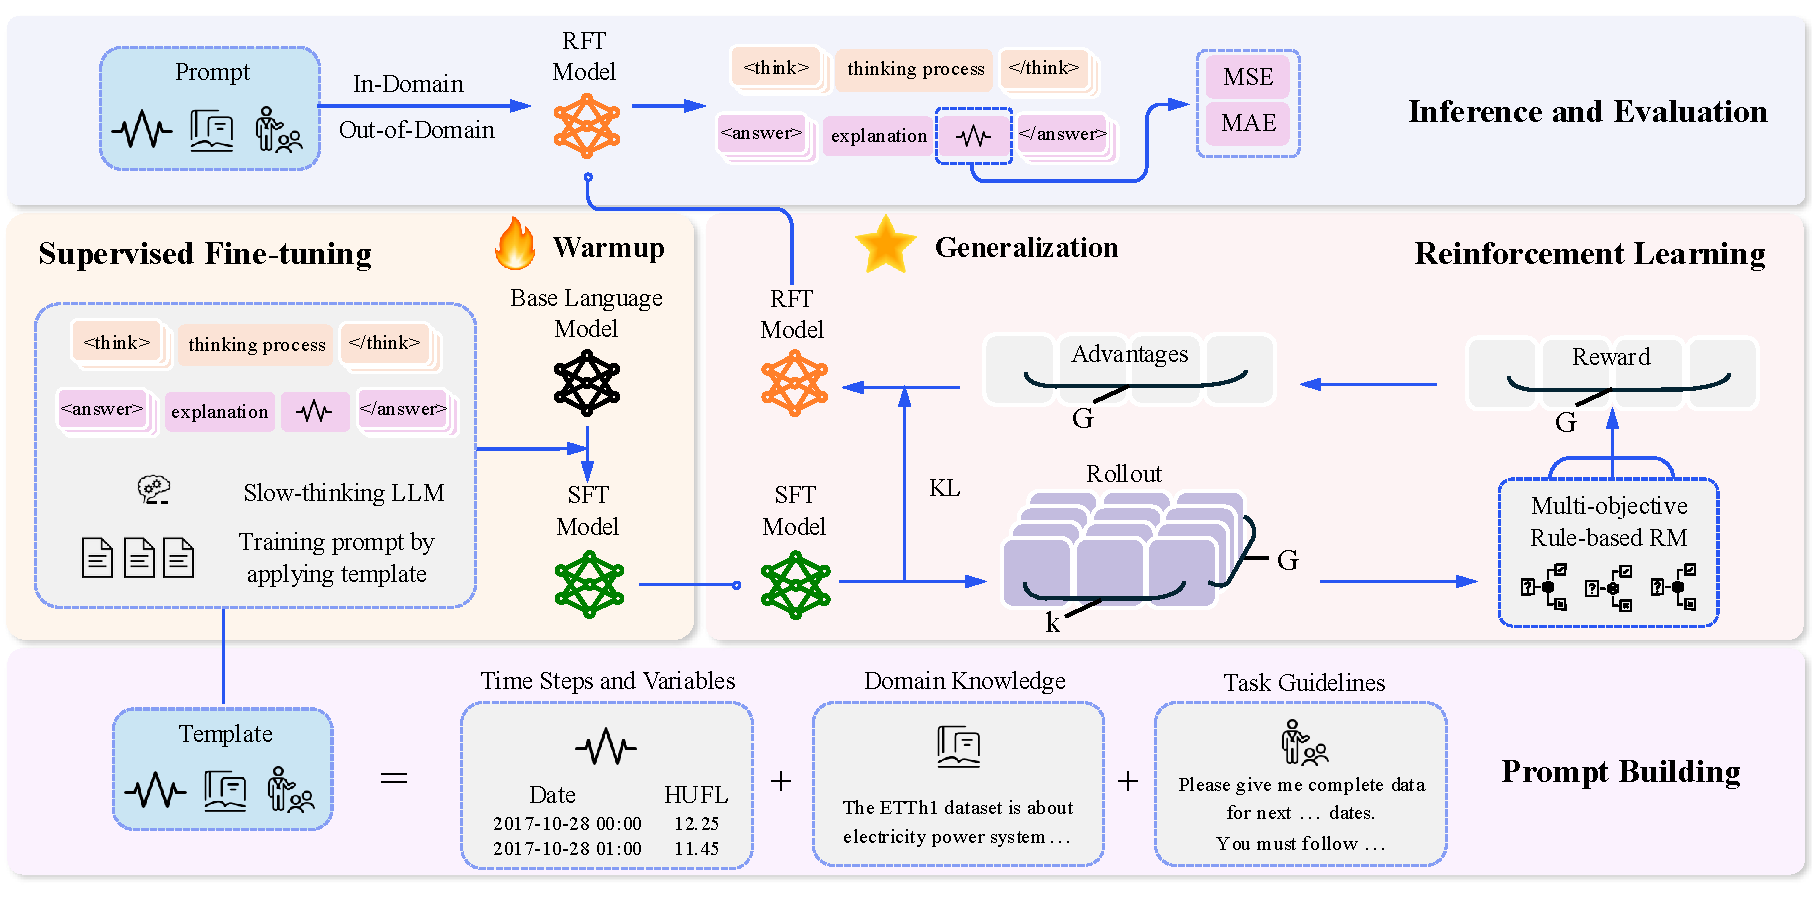
\includegraphics[width=1\textwidth]{images/1_framework_.pdf} 
    \vspace{-0.15in}
    \caption{A diagram illustrating the three steps of \Ours: (1) building a training template with domain context, time steps, and variables, (2) collecting long-CoT data to train a supervised policy, and (3) optimizing the policy via reinforcement learning with group-based relative importance for policy optimization (GRIP) to enhance TSF reasoning capability.} 
    \vspace{-0.06in}
    \label{fig:1_framework} 
\end{figure*}



\subsection{LLMs and Reinforcement Learning}
Reinforcement Learning (RL) \citep{kaelbling1996reinforcement} allows an agent to learn decision-making through interactions with its environment, aiming to maximize cumulative rewards. RLHF introduced RL to LLMs via human feedback \citep{ouyang2022training, kaufmann2023survey}, initially training a reward model on human preferences and then using it for tuning the policy LLM, often with Proximal Policy Optimization.
% However, PPO's complexity due to multiple optimization rounds poses challenges. 
To simplify this, methods like Direct Preference Optimization \citep{rafailov2023direct} and SimPO \citep{meng2024simpo} have been proposed, offering computational efficiency but suffering from off-policy issues \citep{pang2024iterative}. 
Another approach, GRPO \citep{shao2024deepseekmath}, avoids a critic model by estimating baselines from group scores. Following this line, DAPO \citep{yu2026dapo} improves group-based RL with decoupled clipping and dynamic sampling, while GSPO \citep{zheng2025group} performs policy optimization at the sequence level for more stable training. 
Recently, there has been growing interest in combining CoT reasoning with RL to improve reasoning quality and self-refinement in LLMs~\citep{chu2025sft, chen2025sft, song2025r1, li2024getting}. Despite these advances, applying RL to enhance LLM-driven reasoning for time series forecasting tasks remains underexplored in practical, real-world forecasting settings today.


